\documentclass[11pt,a4paper]{article}
\usepackage[utf8]{inputenc}
\usepackage[T1]{fontenc}
\usepackage{amsthm} %numéroter les questions
\usepackage[frenchb]{babel}
\usepackage{datetime}
\usepackage{xspace} % typographie IN
\usepackage{hyperref}% hyperliens
\usepackage[all]{hypcap} %lien pointe en haut des figures
\usepackage[french]{varioref} %voir x p y
\usepackage{fancyhdr}% en têtes
%\input cyracc.def
\usepackage[]{graphicx} %include pictures
\usepackage{pgfplots}
\usepackage[]{circuitikz}
\usepackage{ifthen}

\usepackage[top=1.3 in, bottom=1.3 in, left=1.3 in, right=1.3 in]{geometry} % Yeah, that's bad to play with margins
\usepackage[]{pdfpages}

\usepackage[]{attachfile}

\usepackage{float}
\usepackage{subfig}

\usepackage{todonotes} % \missingfigure
\usepackage{gensymb} % \ohm

\usepackage{framed}

\newdateformat{mydate}{2016--2017}%hack pour remplacer \THEYEAR


\newboolean{corrige}
\ifx\correction\undefined
\setboolean{corrige}{false}% pas de corrigé
\else
\setboolean{corrige}{true}%corrigé
\fi

%\setboolean{corrige}{false}% pas de corrigé

\newboolean{annexes}
\setboolean{annexes}{true}%annexes
%\setboolean{annexes}{false}% pas de annexes

\definecolor{darkblue}{rgb}{0,0,0.5}

\newboolean{mos}
%\setboolean{mos}{true}%annexes
\setboolean{mos}{false}% pas de annexes

\usepackage{aeguill} %guillemets

%% fancy header & foot
\pagestyle{fancy}
%Numero du TP :
\def \labonumber {Projet -- Partie 1}
\lhead{[ELEC-H-310] Choucroute numérique\\ \labonumber}
\rhead{\mydate\today\\ page \thepage}
\chead{\ifthenelse{\boolean{corrige}}{Corrigé}{}}
\cfoot{}
%%

\pdfinfo{
/Author (Quentin Delhaye, Ken Hasselmann, ULB -- BEAMS)
/Title (\labonumber ELEC-H-310)
/ModDate (D:\pdfdate)
}

\hypersetup{
pdftitle={\labonumber [ELEC-H-310] Choucroute numérique},
pdfauthor={Quentin Delhaye, Ken Hasselmann, ULB -- BEAMS},
pdfsubject={}
}

\theoremstyle{definition}% questions pas en italique
\newtheorem{Q}{Question}[] % numéroter les questions [section] ou non []

\newcommand{\reponse}[1]{% pour intégrer une réponse : \reponse{texte} : sera inclus si \boolean{corrige}
	\ifthenelse {\boolean{corrige}} {\paragraph{Réponse :} \color{darkblue}   #1\color{black}} {}
 }

\newcommand{\addcontentslinenono}[4]{\addtocontents{#1}{\protect\contentsline{#2}{#3}{#4}{}}}

\date{\vspace{-1.7cm}\mydate\today}
\title{\vspace{-2cm}\labonumber \\ Digital electronics [ELEC-H-310]\\Design of a cooling control system~: \\ pre-analysis and propeller fan power supply\ifthenelse{\boolean{corrige}}{~\\Corrigé}{}}

%\author{\vspace{-1cm}}%\textsc{Yannick Allard}}

\setlength{\parskip}{0.2cm plus2mm minus1mm} %espacement entre §
\setlength{\parindent}{0pt}






%%%%%%%%%%%%%%%%%%%%%%%%%%%%%%%%%%%%%%%%%%%%%%%%%%%%%%%%%%%%%%%%%%%%%%%%%%%%%%%%%%%%%%%%%%%%%%%%%%%%%%%%%%%%%
%%%%%%%%%%%%%%%%%%%%%%%%%%%%%%%%%%%%%%%%%%%%%%%%%%%%%%%%%%%%%%%%%%%%%%%%%%%%%%%%%%%%%%%%%%%%%%%%%%%%%%%%%%%%%
%%%%%%%%%%%%%%%%%%%%%%%%%%%%%%%%%%%%%%%%%%%%%%%%%%%%%%%%%%%%%%%%%%%%%%%%%%%%%%%%%%%%%%%%%%%%%%%%%%%%%%%%%%%%%
% http://tex.stackexchange.com/questions/128123/circuitikz-current-source
% preparation to create bipoles

\makeatletter
\def\TikzBipolePath#1#2{\pgf@circ@bipole@path{#1}{#2}}

\pgf@circ@Rlen = \pgfkeysvalueof{/tikz/circuitikz/bipoles/length}
\makeatother 

\newlength{\ResUp} \newlength{\ResDown}
\newlength{\ResLeft} \newlength{\ResRight}

% set default dohicky size

\ctikzset{bipoles/doohicky/height/.initial=.4}
\ctikzset{bipoles/doohicky/width/.initial=.6}

% create doohicky shape

\pgfcircdeclarebipole{}
 {\ctikzvalof{bipoles/doohicky/height}}
 {doohicky}
 {\ctikzvalof{bipoles/doohicky/height}}
 {\ctikzvalof{bipoles/doohicky/width}}
 {
    \pgfsetlinewidth{\pgfkeysvalueof{/tikz/circuitikz/bipoles/thickness}\pgfstartlinewidth}
    \pgfextractx{\ResRight}{\northeast}
    \pgfextracty{\ResUp}{\northeast}
    \pgfextractx{\ResLeft}{\southwest}

  \pgfmoveto{\pgfpoint{\ResLeft}{0cm}}
    \pgfpathellipse{\pgfpoint{0.333\ResLeft}{0cm}}{\pgfpoint{0.667\ResRight}{0cm}}{\pgfpoint{0cm}{\ResUp}}
  \pgfmoveto{\pgfpoint{\ResRight}{0cm}}
    \pgfpathellipse{\pgfpoint{0.333\ResRight}{0cm}}{\pgfpoint{0.667\ResRight}{0cm}}{\pgfpoint{0cm}{\ResUp}}
  \pgfusepath{draw} %draw doohicky
    \pgfscope
    \pgfsetarrowsend{latex'}
    \pgfpathmoveto{\pgfpoint{0.667\ResLeft}{1.333\ResUp}}
    \pgfpathlineto{\pgfpoint{0.667\ResRight}{1.333\ResUp}}
    \pgfusepath{draw}   %draw arrow
    \endpgfscope
 }

% create doohicky to-path style

\def\doohickypath#1{\TikzBipolePath{doohicky}{#1}}
\tikzset{doohicky/.style = {\circuitikzbasekey, /tikz/to path=\doohickypath, l=#1}}

% end of setup
%%%%%%%%%%%%%%%%%%%%%%%%%%%%%%%%%%%%%%%%%%%%%%%%%%%%%%%%%%%%%%%%%%%%%%%%%%%%%%%%%%%%%%%%%%%%%%%%%%%%%%%%%%%%
%%%%%%%%%%%%%%%%%%%%%%%%%%%%%%%%%%%%%%%%%%%%%%%%%%%%%%%%%%%%%%%%%%%%%%%%%%%%%%%%%%%%%%%%%%%%%%%%%%%%%%%%%%%%
%%%%%%%%%%%%%%%%%%%%%%%%%%%%%%%%%%%%%%%%%%%%%%%%%%%%%%%%%%%%%%%%%%%%%%%%%%%%%%%%%%%%%%%%%%%%%%%%%%%%%%%%%%%%





















\begin{document}
\pagestyle{empty}
\maketitle
% \vspace*{-1cm}




% ########   ##     ##  ##########  
% ##     ##  ##     ##      ##      
% ##     ##  ##     ##      ##      
% ########   ##     ##      ##      
% ##     ##  ##     ##      ##      
% ##     ##  ##     ##      ##      
% ########    #######       ##      

\section*{Aims}
During three laboratory sessions, you will have to design a small cooling control system based on a propeller fan.
You will also have to be able to interact locally (keyboard) with this system.

During the first lab session, you will first pre-analyse the project in order to isolate the different features required by the project specifications.
Then, you will conceive the speed control of the propeller fan.

\section*{Prerequisite}
Before entering in the lab, you have to read the project specifications defined in the file «~Design of a temperature regulation system~».


\section*{Objectives}
At the end of this lab session, you'll be able to~:
\begin{itemize}
	\item Slice a big amount of project specifications in submodules.
	\item Associate to each module the adequate peripheral devices.
	\item Generate a PWM wave and explain how it works.
\end{itemize}


\newpage


% ########   ##      ##  ##########  ########     #####    
%    ##      ###     ##      ##      ##     ##  ##     ##  
%    ##      ## ##   ##      ##      ##     ##  ##     ##  
%    ##      ##  ##  ##      ##      ########   ##     ##  
%    ##      ##   ## ##      ##      ##   ##    ##     ##  
%    ##      ##     ###      ##      ##    ##   ##     ##  
% ########   ##      ##      ##      ##     ##    #####    


\section{Introduction}
During three laboratory sessions, you will have to design a small cooling control system based on a propeller fan.
You will also have to be able to interact locally (keyboard) with this system.

During the first lab session, you will first pre-analyse the project in order to isolate the different features required by the project specifications.
Then, you will conceive the speed control of the propeller fan.

The pre-analysis phase has a twofold objective : it helps to reinterpretate the project specifications with your words, as well as to push yourselves to slice the problem in simpler subproblems, with only for each a small amount of $\mu$C features.

Moreover, each of these submodule will be easy to reuse in other projects on condition that they are coded so that they are independant from each other.



% #########  ##########  ##     ##  ######     #########  
% ##             ##      ##     ##  ##    ##   ##         
% ##             ##      ##     ##  ##     ##  ##         
% ######         ##      ##     ##  ##     ##  ######     
% ##             ##      ##     ##  ##     ##  ##         
% ##             ##      ##     ##  ##    ##   ##         
% #########      ##       #######   ######     #########  


\section{Preanalysis and reinterpretation of the project specifications}
To simplify the coding, you will first reinterpretate the specifications~:
\begin{itemize}
	\item Generally speaking, what are the features required by the project specifications~?
	Exemple~: pouvoir faire tourner l’hélice à une vitesse réglable.
	\item For each of these features, answer to the following questions~:
	\begin{itemize}
		\item How does the interfacing with external world work~?
		Must external circuits be added~?
		\item What are the inputs and outputs~?
		\item Which $\mu$C peripheral devices are used (you may find some help in the coding guide (guide de programmation))~?
	\end{itemize}
	\item Realise a block diagram showing how those different features interact.
\end{itemize}






% ########   #########   #######   ##            ###      #######   #########  
% ##     ##  ##         ##         ##           ## ##    ##         ##         
% ##     ##  ##         ##         ##          ##   ##   ##         ##         
% ########   ######     ##   ####  ##         ##     ##  ##   ####  ######     
% ##   ##    ##         ##     ##  ##         #########  ##     ##  ##         
% ##    ##   ##         ##     ##  ##         ##     ##  ##     ##  ##         
% ##     ##  #########  ########   #########  ##     ##  ########   #########  


\section{Power supply and speed control of the propeller fan}
This first module that you have to implement is the speed control of the propeller fan, illustrated in figure~\ref{fig:helice}.

\begin{figure}[H]
\center
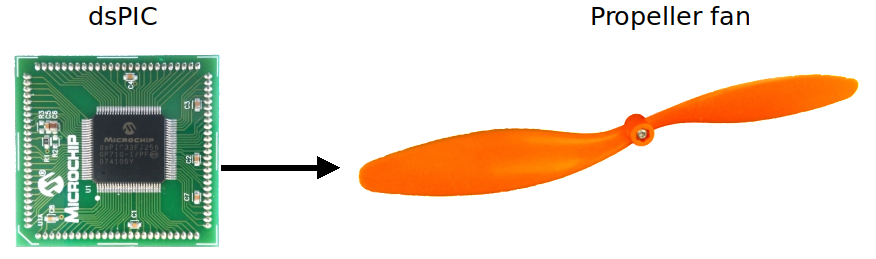
\includegraphics[width=0.8\textwidth]{alim-helice}
\caption{Contrôle de l'hélice par le dsPIC33.}
\label{fig:helice}
\end{figure}

In order to do this, you will have to use the module named \textit{Output Compare -- PWM}, described in the appendix of the dsPIC coding document.

As a reminder, the principle of generating a square wave can be described as being a timer with two thresholds~:
\begin{itemize}
	\item When the timer starts, the ouput pin \texttt{OCx} is at ‘1’.
	\item When the counting register of the timer reaches the first threshold, named \texttt{OCxRS}, the output turns to ‘0’.
	The timer continues to increment.
	\item When the counting register reaches the value of the period \texttt{PRx} , the timer returns zero and the output returns to ‘1’.
\end{itemize}

By playing with the values of these two thresholds, it is possible to generate any square wave.

Operational mode~:
\begin{itemize}
	\item Read the section of the coding guide (guide de programmation) concerning the PWM generator.
	\item Write the routine able to generate on one of the pins \texttt{OCx} a rectangular wave with a period of 100~$\mu s$ and a duty cycle of 40~\%.
	Verify these values with an oscilloscope.
	\item Modify your program so that this routine is presented as a function allowing to change easily the duty cycle without changing the period of the signal.
	\item Connect the power supply pins of the propeller fan at 0V-5V of the protoboard, and connect the input In1 or In2 of the propeller fan to your PWM output.
	Do not forget to connect your grounds together!
	\item Check if the propeller fan rotates with a variable speed.
\end{itemize}






%  #######     #####    ##      ##  ##     ##  #########  ########   ##########  ########    #######    #######   #########  ##     ##  ########   
% ##     ##  ##     ##  ###     ##  ##     ##  ##         ##     ##      ##         ##      ##     ##  ##     ##  ##         ##     ##  ##     ##  
% ##         ##     ##  ## ##   ##  ##     ##  ##         ##     ##      ##         ##      ##         ##         ##         ##     ##  ##     ##  
% ##         ##     ##  ##  ##  ##  ##     ##  ######     ########       ##         ##       #######    #######   ######     ##     ##  ########   
% ##         ##     ##  ##   ## ##   ##   ##   ##         ##   ##        ##         ##             ##         ##  ##         ##     ##  ##   ##    
% ##     ##  ##     ##  ##     ###    ## ##    ##         ##    ##       ##         ##      ##     ##  ##     ##  ##         ##     ##  ##    ##   
%  #######     #####    ##      ##     ###     #########  ##     ##      ##      ########    #######    #######   #########   #######   ##     ##  

\section{PWM as a digital-to-analog converter}
The PWM modulation can be applied to the digital-to-analog conversion.
% Le principe de ce convertisseur est présenté sur la figure suivante.

By eliminating the high frequencis components with a decoupling capacitor, we only keep the mean value of the signal, that is to say $D(t) \cdot 3.3V$, where $D(t)$ is this evolution of the duty cycle over time\footnote{A variant of this principle, known as Delta modulation (or Sigme Delta), is used in analog-to-digital converters with high resolution and low frequency, as well as in the audio sector.}.

\begin{itemize}
	\item Thanks to an oscilloscope, analyse the spectrum of the PWM signal.
	\item In this spectrum, observe the effect of the modulation.
	\item How to size the RC filter to eliminate the switching effect~?
	\item Deduce the limits of this principle~: can we convert any type of signal~?
\end{itemize}


\end{document}
